% $Header: /cvsroot/latex-beamer/latex-beamer/solutions/conference-talks/conference-ornate-20min.en.tex,v 1.7 2007/01/28 20:48:23 tantau Exp $

\documentclass{beamer}

\mode<presentation>
{
  %\usecolortheme[RGB={102,0,15}]{structure}
  %\useoutertheme{infolines}
  %\usetheme{Singapore}
  \setbeamertemplate{items}[ball]
  %\setbeamertemplate{blocks}[rounded][shadow=false] 
  \setbeamertemplate{footline}[page number]
  %\usetheme{Frankfurt}
  % or ...

  \setbeamertemplate{navigation symbols}{}

  %\setbeamercovered{transparent}
  % or whatever (possibly just delete it)
}


\usepackage[english]{babel}
% or whatever

\usepackage[latin1]{inputenc}
% or whatever

\usepackage{times}
\usepackage[T1]{fontenc}
% Or whatever. Note that the encoding and the font should match. If T1
% does not look nice, try deleting the line with the fontenc.
\usepackage{tikz}
\usetikzlibrary{arrows,shapes,automata,shadows}
\usepackage{psfrag}
\usepackage{amssymb,amsmath}
\usepackage{spot}




\title[MAC for mesh] % (optional, use only with long paper titles)
{
Report for evaluation and feedback \\
2012-2016
}


%\subtitle
%{Include Only If Paper Has a Subtitle}

\author[Barcelo] % (optional, use only with lots of authors)
{
Jaume Barcelo
}
% - Give the names in the same order as the appear in the paper.
% - Use the \inst{?} command only if the authors have different
%   affiliation.

\institute[institute] % (optional, but mostly needed)
{
Universitat Pompeu Fabra
}

% - Use the \inst command only if there are several affiliations.
% - Keep it simple, no one is interested in your street address.

\date[date] % (optional, should be abbreviation of conference name)
{
April, 2013, Barcelona
}
% - Either use conference name or its abbreviation.
% - Not really informative to the audience, more for people (including
%   yourself) who are reading the slides online

\subject{}
% This is only inserted into the PDF information catalog. Can be left
% out. 



% If you have a file called "university-logo-filename.xxx", where xxx
% is a graphic format that can be processed by latex or pdflatex,
% resp., then you can add a logo as follows:

%\pgfdeclareimage[height=2cm]{conference-logo}{conference-logo}
%\logo{\pgfuseimage{conference-logo}}



% Delete this, if you do not want the table of contents to pop up at
% the beginning of each subsection:
%\AtBeginSubsection[]
%{
%  \begin{frame}<beamer>{Outline}
%    \tableofcontents[currentsection,currentsubsection]
%  \end{frame}
%}
%\AtBeginSection[]
%{
%  \begin{frame}<beamer>{Outline}
%    \tableofcontents[currentsection]
%  \end{frame}
%}


% If you wish to uncover everything in a step-wise fashion, uncomment
% the following command: 

%\beamerdefaultoverlayspecification{<+->}


\begin{document}
\tikzstyle{every picture}+=[remember picture]

\begin{frame}
  \titlepage
\end{frame}

\begin{frame}{Outline}
  \tableofcontents
  % You might wish to add the option [pausesections]
\end{frame}


% Structuring a talk is a difficult task and the following structure
% may not be suitable. Here are some rules that apply for this
% solution: 

% - Exactly two or three sections (other than the summary).
% - At *most* three subsections per section.
% - Talk about 30s to 2min per frame. So there should be between about
%   15 and 30 frames, all told.

% - A conference audience is likely to know very little of what you
%   are going to talk about. So *simplify*!
% - In a 20min talk, getting the main ideas across is hard
%   enough. Leave out details, even if it means being less precise than
%   you think necessary.
% - If you omit details that are vital to the proof/implementation,
%   just say so once. Everybody will be happy with that.

\section{Collaborators}

\begin{frame}
  \frametitle{Collaborations (not exhaustive list)}
  \begin{columns}[t]
    \column{.5\textwidth}
      \begin{center}
        
\includegraphics[width=0.6in]{figures/boris}
        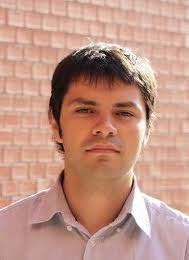
\includegraphics[width=0.6in]{figures/alex}
        
\includegraphics[width=0.6in]{figures/cristina}
        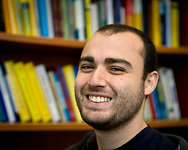
\includegraphics[width=0.6in]{figures/alessandro}
        
        
\includegraphics[width=0.6in]{figures/ken}
        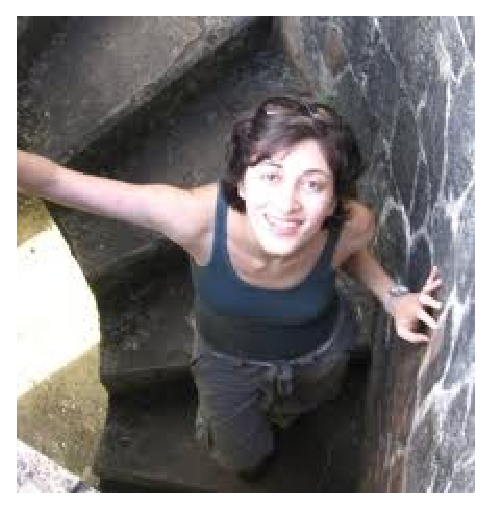
\includegraphics[width=0.6in]{figures/azadeh}
        
\includegraphics[width=0.6in]{figures/nuria}
        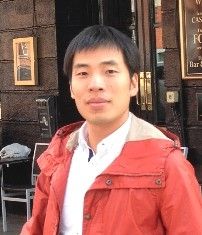
\includegraphics[width=0.6in]{figures/ray}
        
        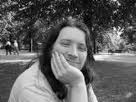
\includegraphics[width=0.6in]{figures/david}
        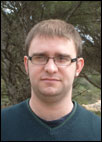
\includegraphics[width=0.6in]{figures/gabriel}
        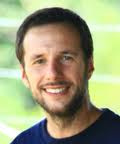
\includegraphics[width=0.6in]{figures/joan}
        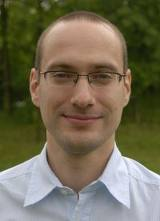
\includegraphics[width=0.6in]{figures/simon}

        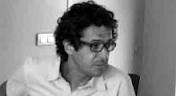
\includegraphics[width=0.6in]{figures/miquel}
        
\includegraphics[width=0.6in]{figures/luis}
      \end{center}
    \column{.5\textwidth}
        \begin{itemize}
          \item Boris Bellalta
          \item Alex Bikfalvi
          \item Cristina Cano
          \item Alessandro Checco
          \item Ken Duffy
          \item Azadeh Faridi
          \item Nuria Garcia
          \item Ruizhi Liao
          \item David Malone
          \item Gabriel Martorell
          \item Joan Melia
          \item Simon Oechsner
          \item Miquel Oliver
          \item Luis Sanabria-Russo
        \end{itemize}
  \end{columns}
\end{frame}

\section{The challenge: Channel access}
\begin{frame}
  \frametitle{Challenges in Medium Access Control (MAC)}
  \begin{columns}[t]
    \column{.3\textwidth}
      \begin{center}
        
\includegraphics[width=1.0in]{figures/wifi}
      \end{center}
      \begin{center}
        
\includegraphics[width=1.0in]{figures/zigbee}
      \end{center}
      \begin{center}
        
\includegraphics[width=1.0in]{figures/rfid}
      \end{center}
    \column{.7\textwidth}
      \begin{block}{}
        \begin{itemize}
          \item successful standards evolve
          \item IEEE 802.11 WiFi WLANs: High speed cost efficient Internet access for mobile devices. Support many devices, offer high throughput, low delay, low jitter. Increase coverage using multi-hop. Efficient use of multiple antennae and channel bonding.
          \item IEEE 802.15.4 ZigBee WSN: Simple, low-power battery devices. Save energy.
          \item EPC Gen2 RFID: Identification and tracking of tags. Read all the tags in a short time.
        \end{itemize}
      \end{block}
  \end{columns}
\end{frame}


\section{Our favorite tool: A decentralized CSP solver}
\begin{frame}
  \frametitle{Our favorite tool: A decentralized CSP solver}
  \begin{columns}[t]
    \column{.5\textwidth}
      \begin{block}{}
        \begin{itemize}
          \item Decentralized resource allocation problems.
          \item A decentralized constraint satisfaction solver.
          \item The only information available to me, as a participant, is whether the constraints I am involved in are satisfied.
          \item Simple. Change your choice if you are not satisfied.
        \end{itemize}
      \end{block}
    \column{.5\textwidth}
      \begin{center}
        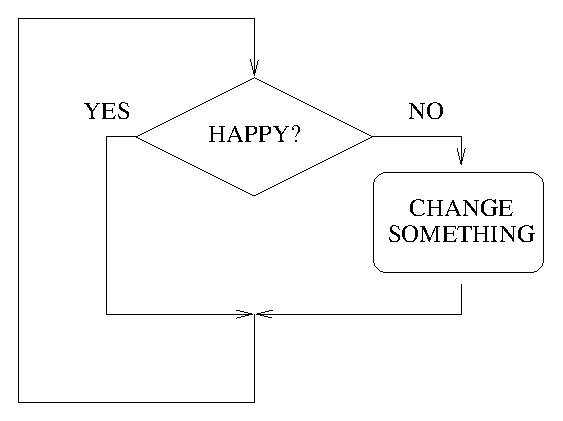
\includegraphics[width=1.5in]{figures/happy}

        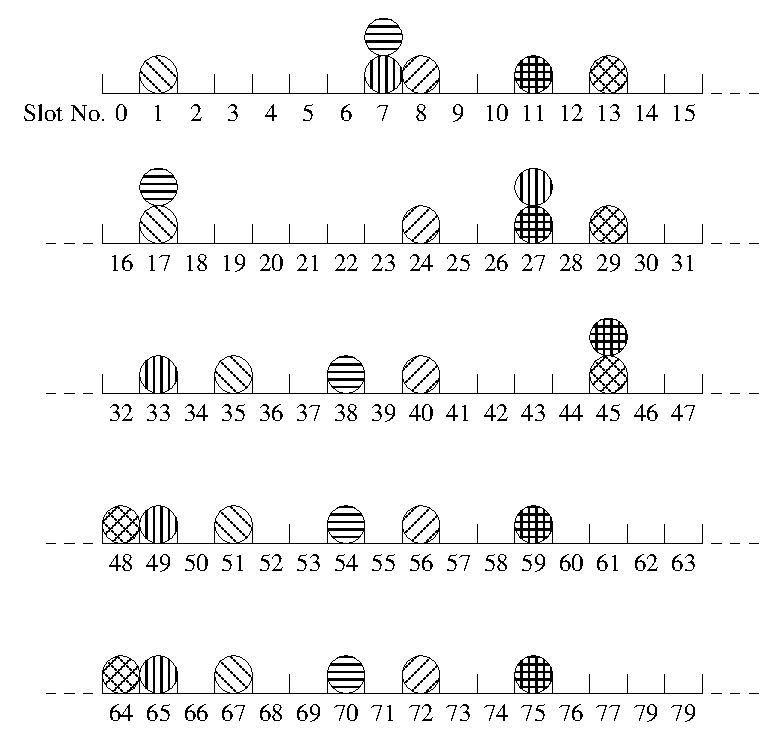
\includegraphics[width=1.8in]{figures/csma_eca_compact}
      \end{center}
  \end{columns}
\end{frame}

\section{First Results}
\begin{frame}
  \frametitle{First Results}
      \begin{block}{}
        \begin{itemize}
          \item \alert<2>{A subtle modification of the IEEE 802.11 protocol to allow collision-free operation in crowded scenarios (backward compatibility preserved, need for more exhaustive evaluation).}
          \item A first solution to achieve collision-free operation in multi-hop wireless mesh networks (still room for improvement).
          \item A model for a simple solver for decentralized constraint satisfaction problems.
          \item Assessment of the performance improvement by collision-free operation when ARF is taken into account.
          \item Evaluation of the impact of queueing processes on MAC protocols supporting MU-MIMO.
          \item USRP spectrum occupancy sensor.
        \end{itemize}
      \end{block}
\end{frame}


\section{An Example}
\begin{frame}
  \frametitle{An Example (not to be explained in detail)}
      \begin{center}
        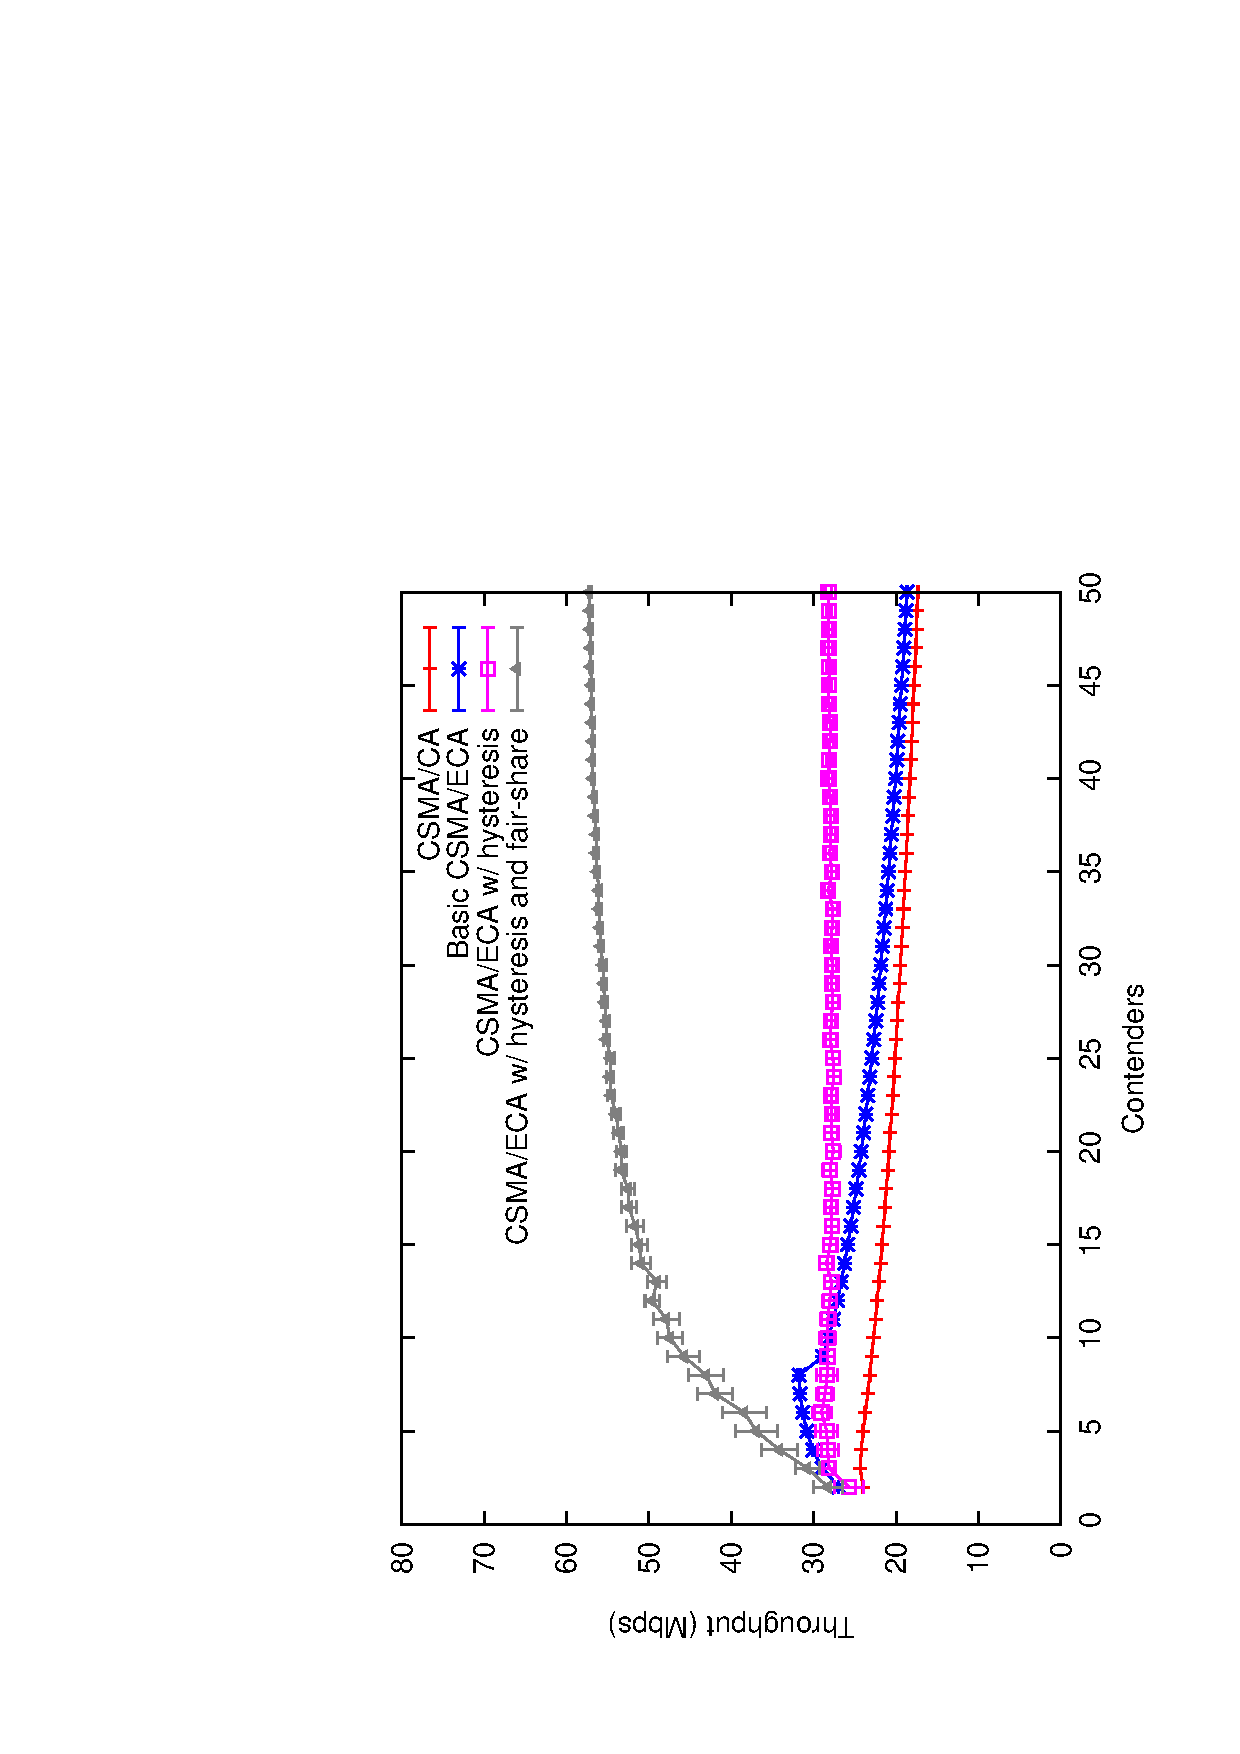
\includegraphics[angle=-90,width=\textwidth]{figures/throughput-combined}
      \end{center}
\end{frame}

\section{Next Steps}
\begin{frame}
  \frametitle{Next Steps}
      \begin{block}{}
        \begin{itemize}
          \item \alert<2>{Trade-offs of frame aggregation.}
          \item Collaboration in the ``Wireless MAC Processors'' front.
          \item Modeling of link activation problem in mesh networks as a decentralized constraint satisfaction problem with sensing restrictions.
          \item Collision-free techniques in RFID contention protocols.
          \item Prototyping with the ``Demo tag''.
          \item QoS in next-gen MAC protocols.
          \item Construction of a collision-free schedule of beacons (WSNs, 802.11s, 802.11p)
        \end{itemize}
      \end{block}
\end{frame}


\section{Projects}
\begin{frame}
  \frametitle{Projects}
      \begin{block}{}
        \begin{itemize}
          \item CISNETs: Collaboration in WSNs.
          \item Commons for Europe. Bottom-up Broadband for Europe.          \begin{itemize}
              \item Create a pool of common resources to be shared by European cities (and citizens).
              \item Grassroots networking initiatives.
              \item High educational value.
              \item Move from a market/competition economy to a commons/collaboration economy (think of wikipedia, open source, creative commons, etc.).
              \item Shift from profit to benefit.
              \item Four pilots: Free Europe WiFi (Nacho), Fiber From The X (Jorge), Mobile Node (Fernando), Open Sensor Network (Alejandro). We involve last year undergrad students in real projects.
          \end{itemize}
          \item Reviewer offer for IP project and CHIST-ERA project proposal.
        \end{itemize}
      \end{block}
\end{frame}

\section{Teaching}
\begin{frame}
  \frametitle{Teaching, coordination and promotion}
      \begin{block}{}
        \begin{itemize}
          \item Opened two undergrad courses. Renewed one.
          \begin{itemize}
              \item QoS
              \item WSN (with Luis) 
              \item Networking Laboratory (with Ray, Alex, Albert)
          \end{itemize}
          \item Graduate seminar on contention protocols.
          \item Two undergrad thesis (Alejandro and Fernando), one Ph.D. thesis (Luis).
          \item Escolab (with Luis and Alejandro).
          \item School's promotional talk.
          \item Degree teaching coordinator (School appointment).
          \item Teaching commission (Department's appointment).
        \end{itemize}
      \end{block}
\end{frame}


\section{External Evaluation}
\begin{frame}
  \frametitle{External Evaluation}
      \begin{block}{}
        \begin{itemize}
          \item Positive evaluation (``Acreditacio de Recerca'', ``agregat'') by the Catalan university quality agency (Agencia per a la Qualitat del Sistema Universitari, AQU).
        \end{itemize}
      \end{block}
\end{frame}

{
\usebackgroundtemplate{\includegraphics[width=\paperwidth]{figures/escolab}}
\begin{frame}[plain]
\end{frame}
}

{
\usebackgroundtemplate{\includegraphics[width=\paperwidth]{figures/mesh}}
\begin{frame}[plain]
\end{frame}
}

{
\usebackgroundtemplate{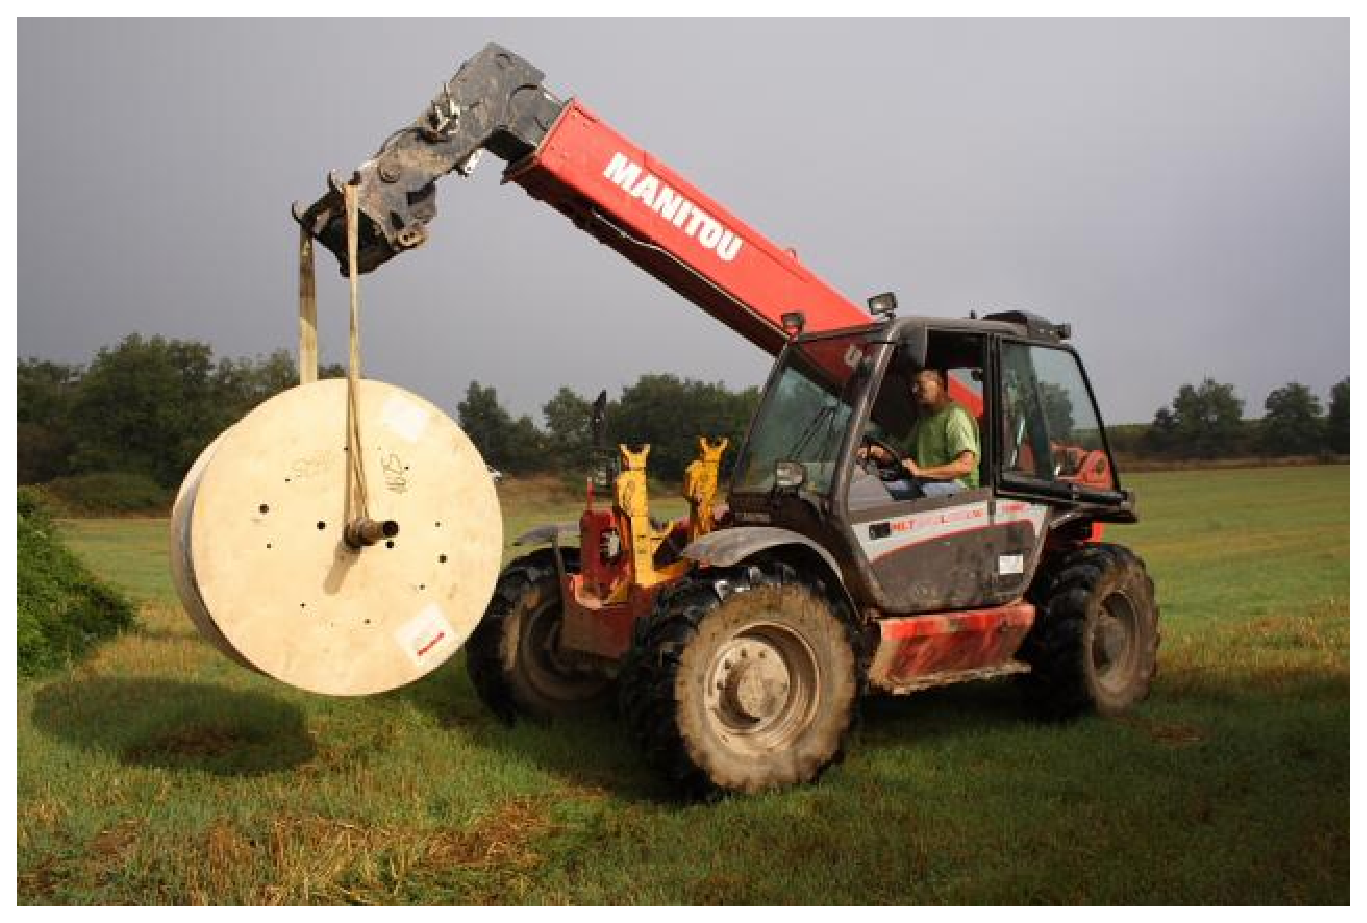
\includegraphics[width=\paperwidth]{figures/bub}}
\begin{frame}[plain]
\end{frame}
}

\begin{frame}{Summary}

  % Keep the summary *very short*.
  \begin{block}{}
        \begin{center}
          \begin{itemize}
            \item Integrated in a research environment.
            \item Some research results. More to be done.
            \item Participation in projects and technology transfer.
            \item Teaching and backing the school and the department.
          \end{itemize}
        \end{center}
  \end{block}
  
  % The following outlook is optional.
  \vskip 1cm
        \begin{center}
          Thank you for your attention. 

        \end{center}
\end{frame}

\end{document}



\begin{frame}{Summary}

  % Keep the summary *very short*.
  \begin{block}{}
        \begin{center}
          \begin{itemize}
            \item Integrated in a research environment.
            \item Some early research results. More to be done.
            \item Participation in projects and technology transfer.
            \item Teaching and backing the school and the department.
          \end{itemize}
        \end{center}
  \end{block}
  
  % The following outlook is optional.
  \vskip 1cm
        \begin{center}
          Thank you for your attention. 

        \end{center}
\end{frame}

\end{document}


